%\documentclass[conference]{IEEEtran}
%\IEEEoverridecommandlockouts
\documentclass{article}
\usepackage[utf8]{inputenc}
\usepackage[%
    left=1.0in,%
    right=1.0in,%
    top=1.0in,%
    bottom=1.0in,%
    paperheight=11in,%
    paperwidth=8.5in%
]{geometry}

% =======================
\usepackage{xeCJK}
\usepackage{amssymb}
\usepackage{amsmath}
\usepackage{amstext}
\usepackage{amsopn}
%\usepackage{algorithmic}
\usepackage{graphicx}
\usepackage{textcomp}
\usepackage{xcolor}

\usepackage{textcomp}

\usepackage{boxedminipage}
\usepackage{enumerate}
\usepackage{multirow}
\usepackage{url}
\usepackage{times}
\usepackage{version}
% \usepackage[pdftex]{graphicx}
\usepackage{epsfig}
\usepackage{epsf}
%\usepackage{graphics}
\usepackage{caption}
\usepackage{subfigure}
\usepackage{algorithm}
\usepackage{algpseudocode}
%\PassOptionsToPackage{bookmarks={false}}{hyperref}
%%%%%%%%%%%%
\usepackage{comment}
\usepackage{multicol}
\usepackage{booktabs}
\usepackage{dblfloatfix}
% ==========================

\setCJKmainfont[Path=fonts/]{msjh.ttc} % 中文字型
\setCJKmonofont[Path=fonts/]{msjh.ttc} % 中文等寬字型
\usepackage{enumitem}

\begin{document}

\title{E-Healthcare Management System}
\author{
  Cheng-Han Hsieh, 謝承翰\\
  \texttt{B103040012}
  \and
  Shih Yu Sun, 孫世諭\\
  \texttt{B103040001}
  \and
  Casper Liu, 劉世文\\
  \texttt{B093040051}
  \and
  Tina Tsou, 鄒宜庭\\
  \texttt{B096060032}
  \and
  Chia-Yen Huang, 黃嘉彥\\
  \texttt{B103040051}
  \and
  Ting-Hao Hsu, 許廷豪\\
  \texttt{B103040008}
}

\maketitle

\section{Outline}
\label{sec:outline}

\begin{figure}[h]
  \centering
  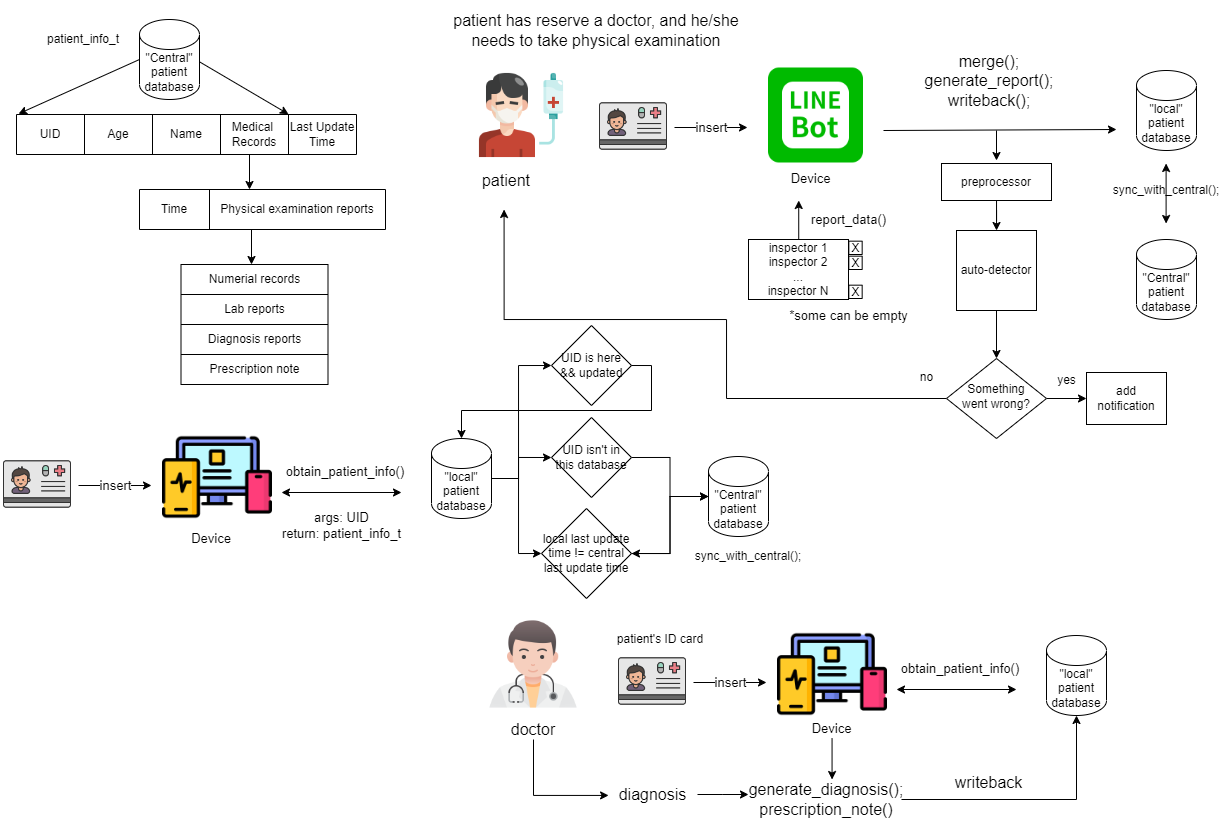
\includegraphics[scale = 0.3]{asset/flowchart.png}
  \caption{A simple example of outline.}
  \label{fig:flowchart}
\end{figure}


\section{Features}
\label{sec:features}

With this E-healthcare management system, the hospital/clinic can easily 
sync the information of patients with other health systems, manage 
the information of patients.
For patients, the patient can do most of the things online, for example, 
make a doctor appointment, look up the medical records and prescriptions, 
and obtain the physical reports at home. Even more, the system use machine 
learning to detect the abnormal data in the reports, notify the patient 
to prevent the disease becoming worse. 
To conclusion, the major features of the system can be summarized as 
followings: 
\begin{itemize}
  \item Automatically sync the information of patients between different health systems by using local and central database. 
  \item Facilitate the accessing of medical records and prescriptions, for both doctors and patients. 
  \item Introduce the automatic disease detecters by leveraging machine learning and big data. 
\end{itemize}

\section{Methodology}
\label{sec:methodology}

\subsection*{Database}
\begin{figure}[h]
  \centering
  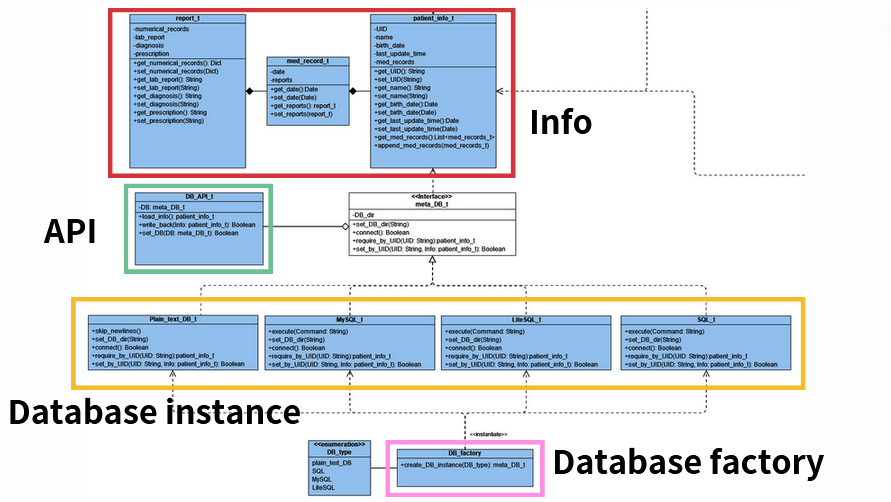
\includegraphics[scale = 0.7]{asset/DB_UML.png}
  \caption{The UML of the whole database.}
  \label{fig:DB_UML}
\end{figure}
\begin{figure}[h]
  \centering
  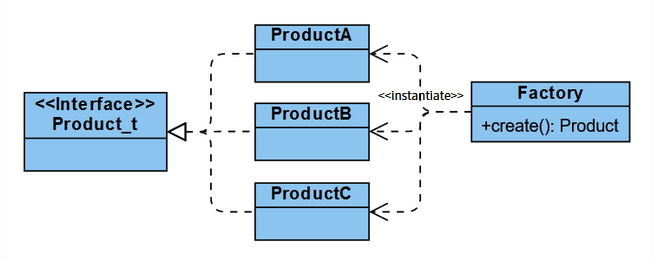
\includegraphics[scale = 0.7]{asset/simple_factory.png}
  \caption{The UML of a simple factory.}
  \label{fig:simple_factory}
\end{figure}

\subsection*{Frontend and Medium}

\begin{figure}[h]
  \centering
  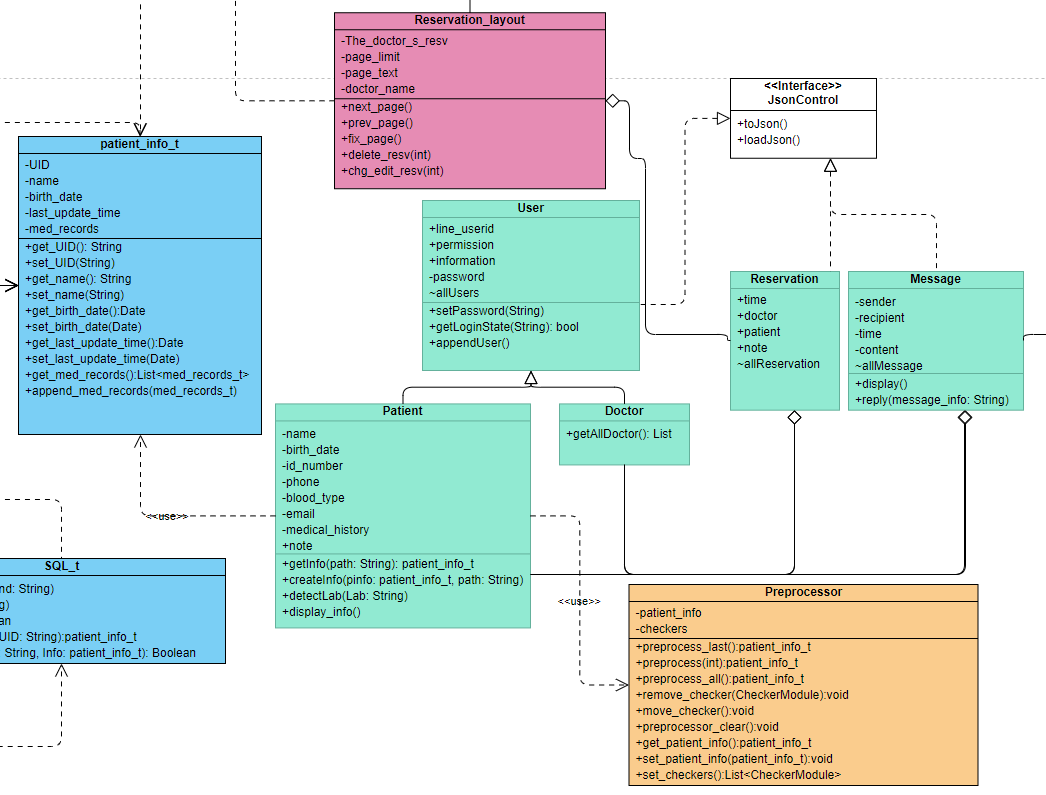
\includegraphics[scale = 0.5]{asset/MED_whole.png}
  \caption{The UML of frontend and medium.}
  \label{fig:uml_frontend_and_medium}
\end{figure}

In the code for the patient frontend and middleware, our functionalities are as follows (refer to Figure \ref{fig:uml_frontend_and_medium}):

\begin{enumerate}[label=\arabic*.]
    \item Utilize Ngrok to forward external requests to the locally specified port.
    \item Integrate LineBot, HTML, JS, and CSS, serving as the patient frontend to send requests such as registration, message sending, and reservations.
    \item Connect to the database to retrieve detailed information based on the user's ID.
    \item Interface with the Processor (Lab), sending detailed information retrieved from the database to the C++ Processor (Lab) for processing and receiving the information back.
    \item Enable the Doctor GUI to utilize the Patient Class to 
    \begin{enumerate}[label=(\roman*)]
        \item obtain detailed information from the database,
        \item access return information from the Processor (Lab),
        \item retrieve the Message Class, and
        \item use the \texttt{Reply()} method to quickly respond to messages via LineBot (refer to Figure \ref{fig:uml_frontend_and_medium}),
        \item obtain detailed data from the Reservation Class,
        \item access the Doctor Class, and
        \item verify its name and password for login.
    \end{enumerate}
\end{enumerate}

Next, we will explain each class in the frontend and medium, highlighting some special member functions and attributes:

\subsubsection*{User}

\begin{itemize}
    \item An abstract class primarily responsible for handling account information such as:
    \begin{enumerate}[label=(\roman*)]
        \item \textbf{permission:} Manages permissions, used to confirm the current user mode (admin or guest).
        \item \textbf{line\_id:} Mainly used to record the user's Line ID, this information is automatically obtained from Line during registration and transmitted to our server.
        \item \textbf{getLoginState(String):} Takes a password as input and checks if it is the correct password.
    \end{enumerate}
\end{itemize}

\subsubsection*{Patient}

\begin{itemize}
    \item A child class of User, mainly deals with patient account information, where it interfaces with the \texttt{patient\_info\_t} in the database to obtain detailed data such as heart rate, blood glucose:
    \begin{enumerate}[label=(\roman*)]
        \item \textbf{detectLab(String):} Will send the information of \texttt{patient\_info\_t} to the Preprocessor, obtaining a detailed diagnosis such as "high heart rate," "diabetes risk," etc (refer to Figure \ref{fig:uml_medium_preprocessor_database}).
    \end{enumerate}
\end{itemize}

\begin{figure}[h]
  \centering
  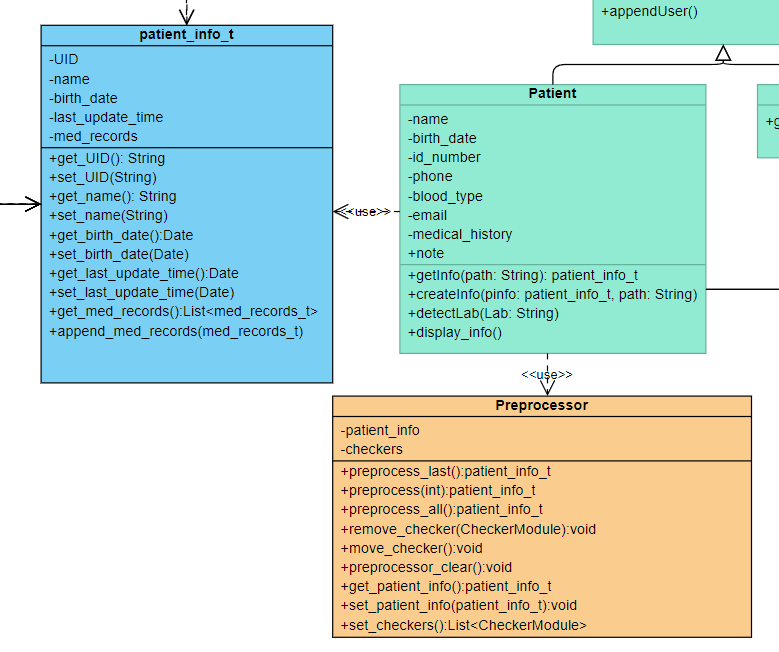
\includegraphics[scale = 0.5]{asset/MED_usage_processor_DB.png}
  \caption{The UML of interaction between medium, preprocessor and database.}
  \label{fig:uml_medium_preprocessor_database}
\end{figure}

\subsubsection*{JsonControl}

\begin{itemize}
    \item An interface implemented by the User, Reservation, and Message classes. Its main purpose is to serialize objects into JSON files for easy storage and access:
    \begin{enumerate}[label=(\roman*)]
        \item \textbf{toJson():} Stores all objects of the entire class in JSON format.
        \item \textbf{loadJson():} Reads a JSON file and restores all objects from it into a list.
    \end{enumerate}
\end{itemize}

\subsubsection*{Reservation}

\begin{itemize}
    \item When a patient uses the frontend LineBot to make a reservation, a Reservation object is created. It is used and deleted by the Doctor GUI and includes Patient and Doctor objects to determine the patient and the reserved doctor (refer to Figure \ref{fig:uml_medium_and_doctor_gui}).
\end{itemize}

\subsubsection*{Message}

\begin{itemize}
    \item When a patient uses the frontend LineBot to send a message, a Message object is created. It is used, replied to, and deleted by the Doctor GUI and includes Patient and Doctor objects to determine the patient and the doctor being messaged (refer to Figure \ref{fig:uml_medium_and_doctor_gui}):
    \begin{enumerate}[label=(\roman*)]
        \item \textbf{reply():} Based on its own Patient object, it uses LineBot to send a message back to the patient (because the Patient object contains the line\_id attribute).
    \end{enumerate}
\end{itemize}

\begin{figure}[h]
  \centering
  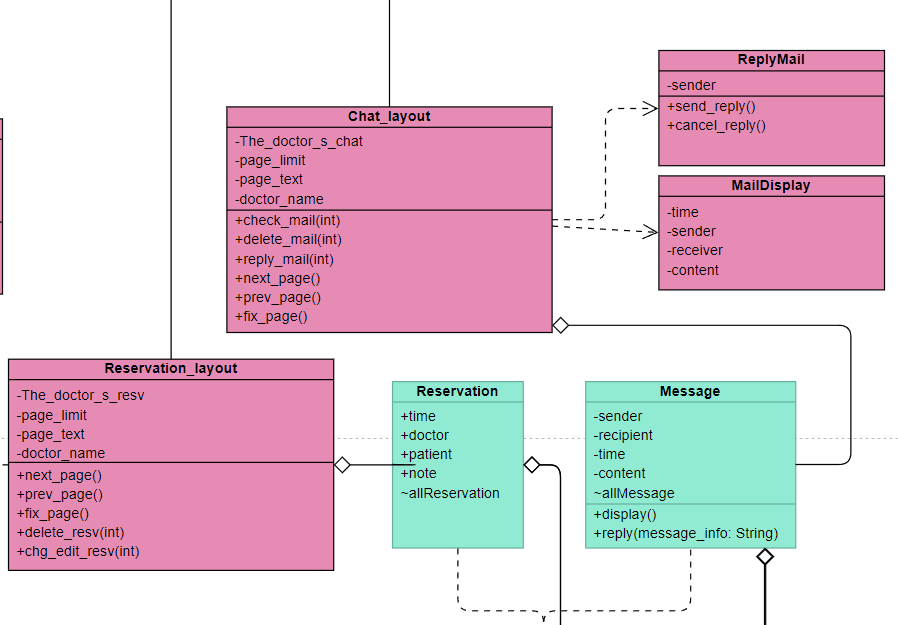
\includegraphics[scale = 0.5]{asset/MED_usage_doctor_gui.png}
  \caption{The UML of interaction between medium and Doctor GUI.}
  \label{fig:uml_medium_and_doctor_gui}
\end{figure}



\section{Code}
\label{sec:code}

\section{Conclusion}
\label{sec:conclusion}

\section{Contribution}
\label{sec:contribution}

\end{document}